

\setcounter{section}{3}
\section{Hardware Design}
\bigskip
\subsection{System Operation Modes}
\medskip
The Akrievia Beacon system will have two modes of operations, idle mode and emergency mode. Idle mode occurs during every day operation that is not under an emergency disaster. An emergency disaster is defined as a situation that poses an immediate risk to health, life, property, or environment. Most emergency disasters require urgent intervention to prevent a worsening of the situation. In emergency disaster situations the system will be triggered on to operate under the emergency mode following the system state diagram as shown in figure \ref{sys_state}.

\bigskip
When system is under idle mode, the beacon system does not attempt to transmit location information from ID Tags to the DPU, as the ID Tags will be under deep sleep mode with the transceiver powered off. In idle mode the system is available for configurations such as adding, editing, and deleting ID Tags, beacons and blueprints. In the Event of an emergency, a trigger such as one that could be associated with a fire alarm will trigger the Akriveia Beacon system state into the emergency mode.

\bigskip
When system is under emergency mode, the beacons will attempt to establish a data pipeline using the UWB modules. And the ID Tags are triggered on by personnel carrying the device that are in need of rescue or assistance. Under emergency mode the DPU triggers the Beacons to start sending and receiving packets to determine ToF data from the ID Tags. The ID tags will receive request packet from beacon and transmit location data back to the beacon. Once the emergency situation is resolved the system can be switched back into idle mode by privileged administers.

\medskip
\begin{figure}[H]
\centering
    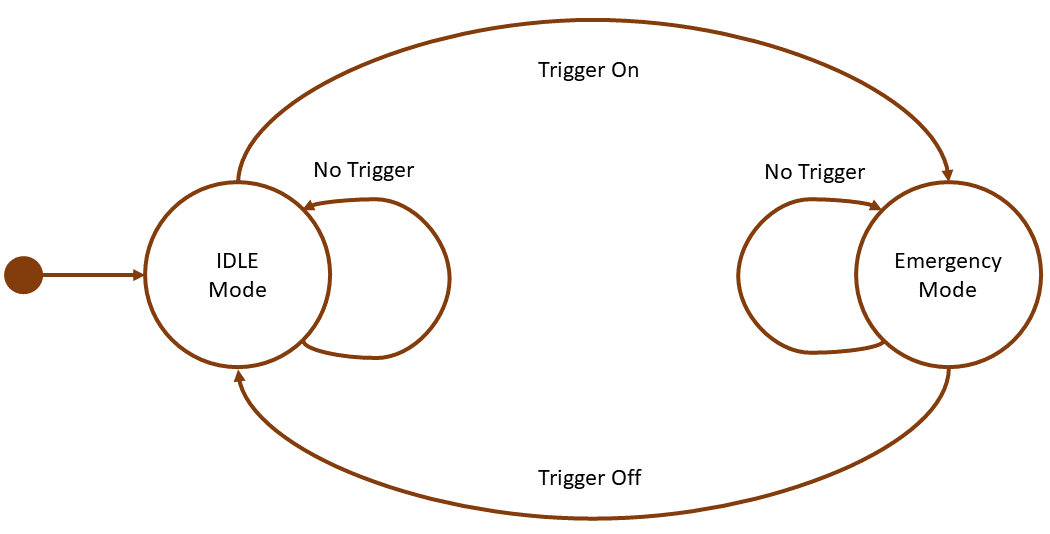
\includegraphics[width=\linewidth]{./images/state_d.png}
    \caption{Akriveia Beacon System State Diagram}
    \label{sys_state}
\end{figure}
\medskip



\pagebreak
\subsection{Communication Protocol}
\subsubsection{Beacon to ID Tag Communication}
\medskip
Communication between beacon and ID tag is facilitated on layer 1 the Physical (PHY) layer of the Open Systems Interconnection model (\Gls{OSI} model). The Physical layer is responsible for converting data into bits for transmission and converting received bits back into data. The logical connection formed between the two entities are the radio channels that are present in air. In the proof of concept phase, 2MHz wide BLE advertising channels 37, 38 and 39 with center frequencies at 2402MHz, 2426MHz and 2480MHz respectively can be used \cite{R4-2-3}. In the engineering prototype and final product phase, 500MHz wide UWB channels 1, 2, 3 and 5 with center frequencies at 3494MHz, 3993MHz, 4492MHz and 6489MHz respectively can be used \cite{R4-2-2}. The difference in frequency and power spectral density can be observed by the plot below (figure \ref{spectrum}). The radio channels will be used at full duplex to allow simultaneous transmission in both sending and receiving directions. Digital data such as RSSI measurements, ToF measurements and MAC address are encoded into analog signals by means of modulation to represent the data with continuously varying electromagnetic waves. Modulation in both BLE and UWB form pulses of analog signals prior to transmission \cite{R4-2-3}. The process of sending and receiving these analog signals are handled by the integrated chip antenna of the ESP32 and DWM1000 modules. Upon reception of the analog signals, the receiver's demodulator and decoder will reverse the work of the sender to retrieve the digital data. 

\bigskip
\begin{figure}[H]
\centering
    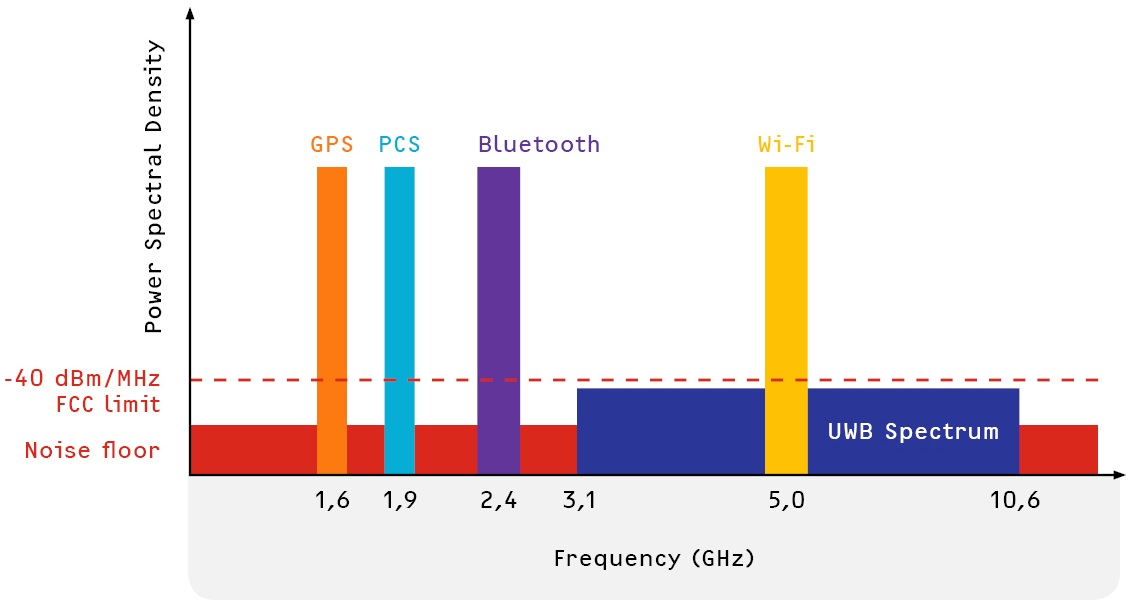
\includegraphics[width=\linewidth]{./images/spectrum.jpg}
    \caption{Common Signal Power spectral Density VS Frequency}
    \label{spectrum}
\end{figure}

\pagebreak
\subsubsection{Beacon to DPU Communication}
\medskip
For the proof of concept and prototype, data-pipeline is a simple implementation with the serial interface. The Beacons will receive and send data with the data processing unit over the USB serial read and write interface. In the Final design the Beacons will use the WiFi module on the ESP32 to join a privately hosted access point created by a hostapd on the data processing unit (Raspberry Pi). \Gls{Hostapd} (Host access point daemon) is a user space software access point capable of turning normal network interface cards into access points and authentication servers. The current version supports Linux (Host AP, madwifi, mac80211-based drivers) and FreeBSD (net80211) \cite{R4-1-2-1}. Once each beacon is connected to the access point they will be assigned an IP by the Dynamic Host Configuration Protocol (\Gls{DHCP}) server. A one-to-many network will be created as shown in figure 2. Using User Datagram Protocol (UDP) communication over the networking layer (layer 2-3 on OSI model), the DPU can bind on the gateway IP and a specific port to listen for forwarded beacon data. To initiate control with the beacons, the DPU will bind to each beacon IP at a specified port and send commands via UDP.

\medskip
\begin{figure}[H]
\centering
    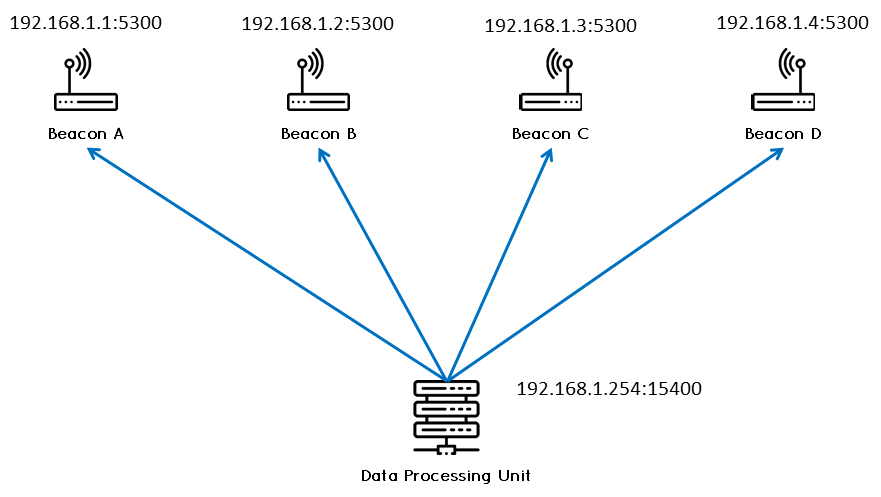
\includegraphics[width=\linewidth]{./images/UDP.png}
    \caption{UDP Communication Network}
    \label{udp}
\end{figure}
\medskip



\pagebreak
\subsection{Beacon Design}
\medskip
To control the beacons the DPU will send a command to the beacon and the ESP32 will evaluate the command and execute accordingly as shown in the beacon flow diagram in figure \ref{bcn_flow}. When system is under emergency mode, the DPU initiates a start command to the Beacons. Once the Beacons acknowledges the start request, it attempts to establish data pipelines to each of the ID Tags in range of the UWB transceiver. After a successful connection, ToF data between beacon and ID tag will be collected and forwarded to the data processing unit for trilateration calculation and error processing before displaying to the user via GUI. On the DPU data of each id tag encountered will be stored in a hash table entry, with the \Gls{MAC} address of each ID tag as the key. The distance measurement are store a rolling buffer for each id tag so that data points can be averaged, reducing estimation error.\\

\bigskip
\begin{figure}[H]
\centering
    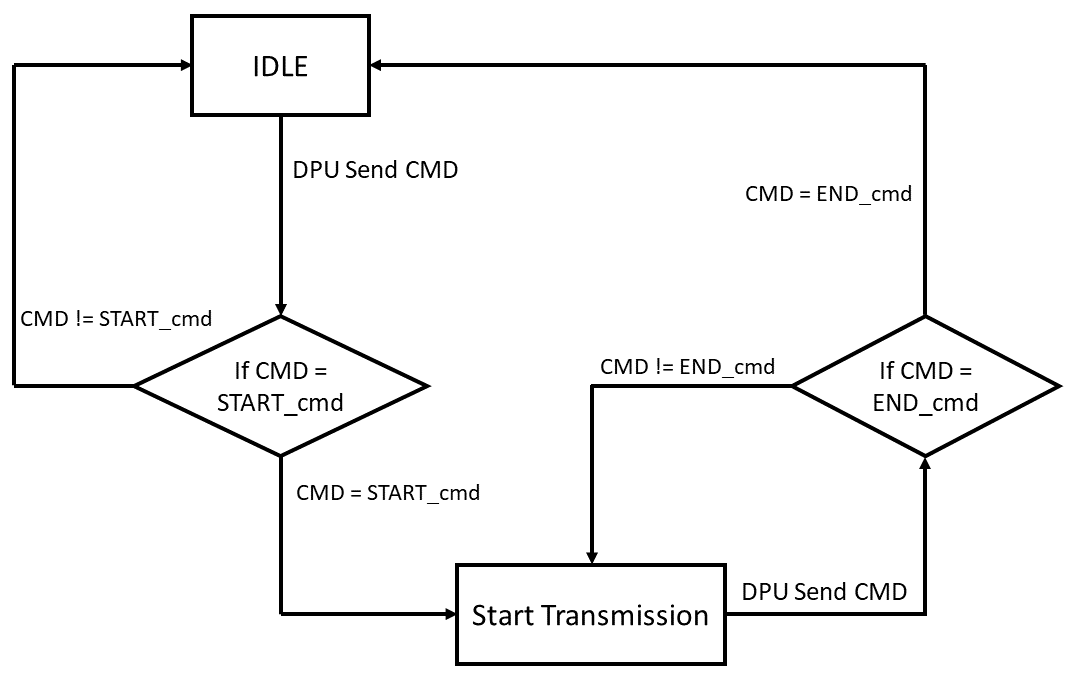
\includegraphics[width=\linewidth]{./images/beacon_flow.png}
    \caption{Beacon System Flow Diagram}
    \label{bcn_flow}
\end{figure}
\medskip

\pagebreak
A 3D appearance mock-ups of the ID Tag was done in Solidworks and can be seen in the Computer Aided Design (CAD) representation, figure \ref{Bcn_CAD}. The Beacon units, which will relay location data from the ID Tags to the Data Processing Unit (DPU), consist of an ESP32 module, a DWM1000 UWB transceiver, a 9V lithium ion battery, and a power cable. These components of the device will be contained in an encasing made from \Gls{PLA} plastic. Each beacons will have LEDs indicating the power and transmission state, and a reset button for resetting the device state. 

\bigskip
\begin{figure}[H]
\centering
    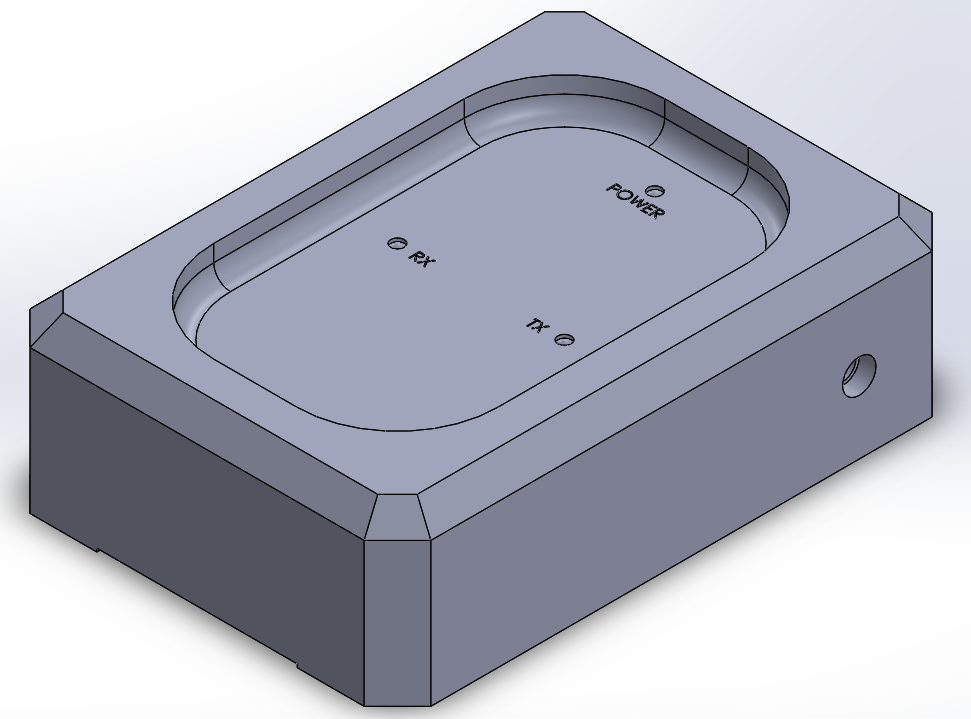
\includegraphics[width=\linewidth]{./images/Beacon.png}
    \caption{CAD representation of Beacon}
    \label{Bcn_CAD}
\end{figure}



\pagebreak
\subsection{ID Tag Design}
\medskip
The ESP32 is used in the ID tag as it contains a function called deep sleep mode, in which the ID Tag has minimum power consumption and does not transmit data for location tracking. During idle mode, the ID tags are operating under deep sleep mode for power conservation drawing only 10uA of current. Therefore, real time tracking outside of emergency mode is not possible as insufficient power is provided to the DWM1000 modules. The ID Tag will be activated in an emergency situation via capacitive touch button located on the device. As user wake the ID tags by triggering the touch button the ID tags will attempt to connect to the Beacons. If the system is not in an emergency state, the ID Tag will fail to establish a connection and briefly show the charge level before returning to deep sleep mode. If system is under the emergency mode, the MCU on ID tags will be able to establish a data pipeline with the beacons on specified UWB channel, and the ID tag will then transmit an acknowledge packet back to the beacon to produce location data as described in the system flow diagram in figure \ref{id_flow}. Only during active emergency mode will the beacons be requesting for establishment of data pipeline and to initiate DWM1000 Ranging state.

\bigskip
\begin{figure}[H]
\centering
    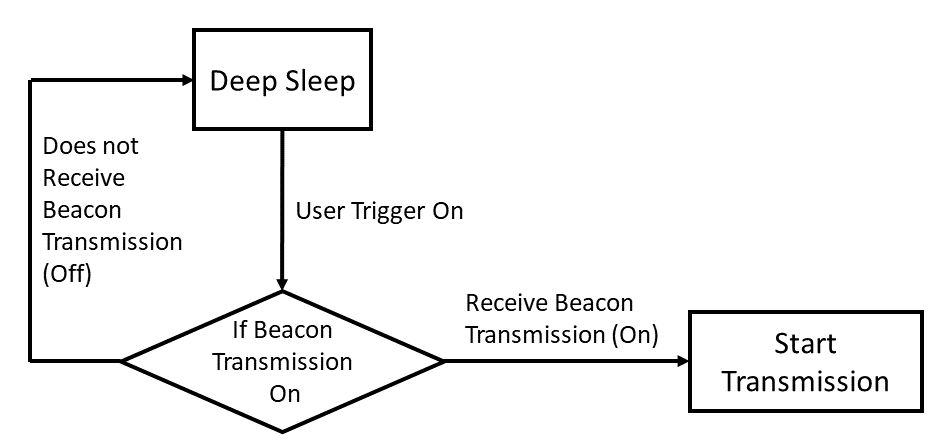
\includegraphics[width=\linewidth]{./images/id_flow.png}
    \caption{ID Tag System Flow Diagram}
    \label{id_flow}
\end{figure}

\pagebreak
A 3D appearance mock-ups of the ID Tag was done in Solidworks and can be seen in the CAD representation, figure \ref{ID_Tag}. The ID Tags, the part of the system being tracked by the Beacons, will be powered by a rechargeable 4-5 V battery with minimal 3000mAH, which will be charged over time by a RF harvester (see sec. 5.2). The ID Tag will consist of an ESP32 MCU module, and a DWM1000 UWB transceiver chip. The internal components of the ID Tag will be contained in a \Gls{PLA} plastic shell with LEDs indicating the power state and transmission activity of the ID Tag. 

\bigskip
\begin{figure}[H]
\centering
    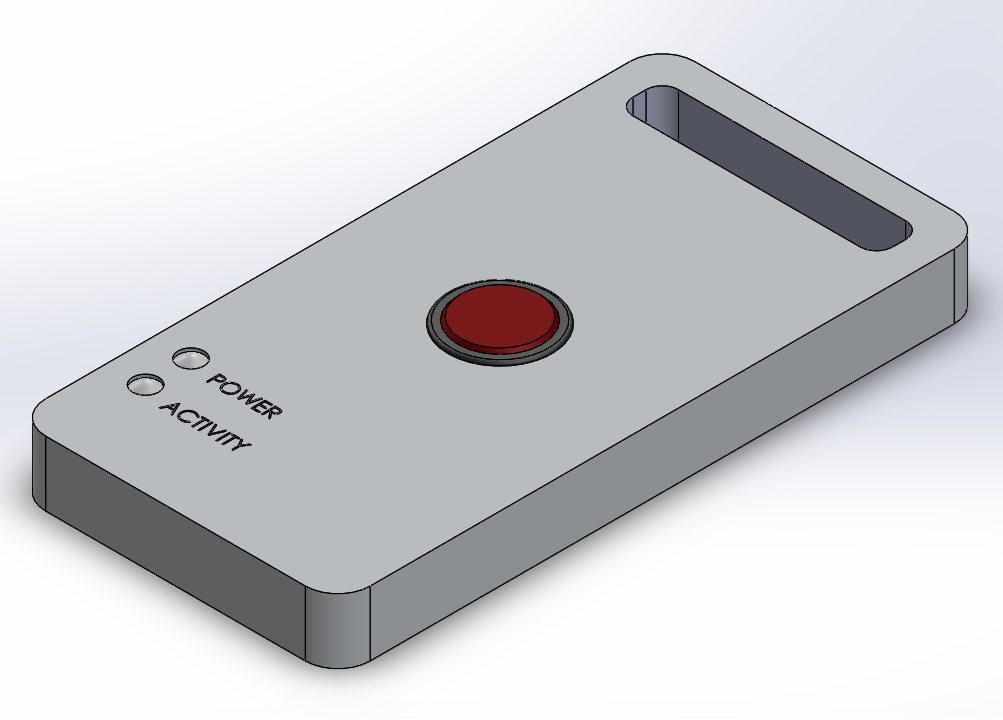
\includegraphics[width=\linewidth]{./images/ID_Tag.png}
    \caption{CAD representation of ID Tag}
    \label{ID_Tag}
\end{figure}



\pagebreak
\subsection{Hardware Design Specification}
\medskip
TRIWAVE SYSTEMS has chosen to develop the proof-of-concept prototype using 2.4GHz Bluetooth radio modules for initial testing of the overall system feasibility and the accuracy of the trilateration method. The system will then be improved upon by incorporating Decawave DWM1000 Ultra-Wideband (UWB) modules for further prototyping. ESP32 Micro-controller Units (MCUs) will be used to control the beacons and ID tags and a Raspberry Pi 3 B+ will be used as a data processing unit. The requirements below detail the requirement for hardware functionality of the Akrivia Beacon system.

\medskip
\bgroup
\def\arraystretch{1.5}
\begin{table}[H]
\centering
\begin{tabular}{ | m{3cm} | m{12.5cm} |}
\hline
\textbf{REQ.HW.1 - C} & The Beacons must use ESP32 as the microcontroller unit and transceiver \\
\hline
\textbf{REQ.HW.2 - C} & The ID Tag must use ESP32 as the microcontroller unit and transceiver \\
\hline
\textbf{REQ.HW.3 - P} & ID tag broadcast duration must be at least 1 hour long upon activation\\
\hline
\textbf{REQ.HW.4 - P} & ID tag must return to deep sleep mode after broadcasting period\\
\hline
\textbf{REQ.HW.5 - P} & The Beacons must use Decawave DWM1000 UWB modules as transceivers\\
\hline
\textbf{REQ.HW.6 - P} & The Beacons must use ESP32 as the controller units\\
\hline
\textbf{REQ.HW.7 - P} & The ID tags must use Decawave DWM1000 UWB modules as transceivers\\
\hline
\textbf{REQ.HW.8 - P} & The ID tags must use ESP32 as the controller units\\
\hline
\end{tabular}
\caption{Hardware Design Specification}
\end{table}


